\chapter{Experiments}\label{ch:Experiments} 
In this chapter, we will focus on some experiments that we performed and their results.
In the first part, we show the images that were used for the experiments. Afterwards we are going
to tackle the point of parameter selection since it is not trivial to find the optimal set of
parameters. Therein, we explain the meaning of each parameter in both the corner detection and
inpainting process as well as present a reasonable choice for them.
Lastly, we present some results from the experiments and whether or how this is useful for
PDE-based image compression methods.
\section{Test images}
We divide the test images in 2 different groups because as we will see later in this chapter, the
method works better on a certain category of images.
First, we have the `normal' grey value images as seen in figure \ref{fig:GreyValueImg}. All these
images were provided by Joachim Weickert and count to the standard test images in the image
processing community.
The second groud is the group of binary grey value images, i.e. images that contain only black and
white pixels instead of 256 different grey values as is the case in the first category. Of this
second category (cf. figure \ref{fig:BinaryImg}), only the picture \texttt{cat} was provided by
Joachim Weickert, the other ones were generated by me using the image manipulation programme
\texttt{GIMP}. Each of these generated pictures was created to test or highlight different aspects
of the corner detection or inpainting method as seen in section \ref{sec:Results}.
\begin{figure}[ht]
    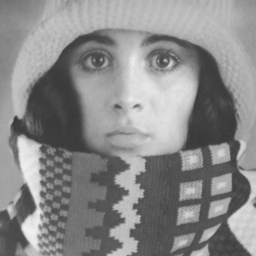
\includegraphics[width=0.5\linewidth]{../../images/grey/trui.png}
    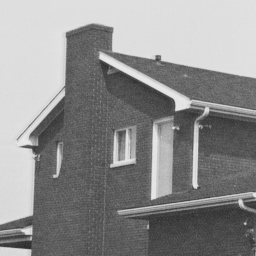
\includegraphics[width=0.5\linewidth]{../../images/grey/house.png}
    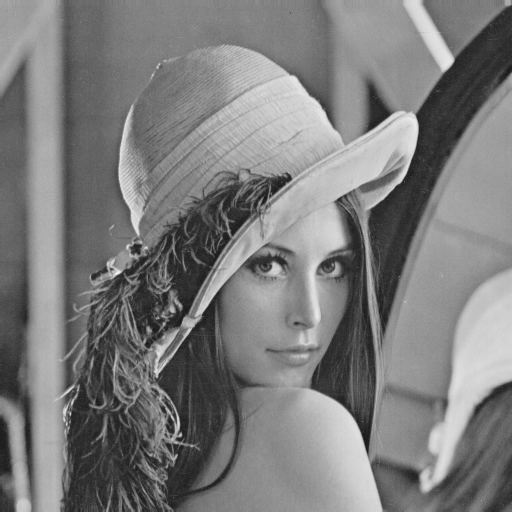
\includegraphics[width=0.5\linewidth]{../../images/grey/lena512.png}
    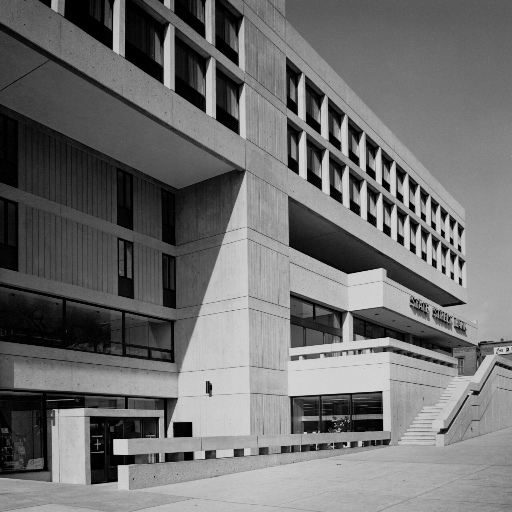
\includegraphics[width=0.5\linewidth]{../../images/grey/bank.png}
    \caption{Grey value images used for testing. From left to right and from top to bottom: \texttt{trui},
    \texttt{house}, \texttt{lena512}, \texttt{bank}}\label{fig:GreyValueImg}
\end{figure}
\begin{figure}[ht]
    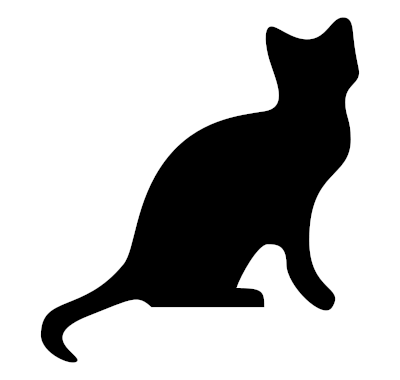
\includegraphics[width=0.32\linewidth]{../../images/binary/cat.png}
    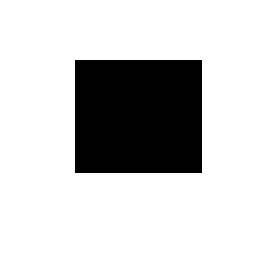
\includegraphics[width=0.32\linewidth]{../../images/binary/rect.png}
    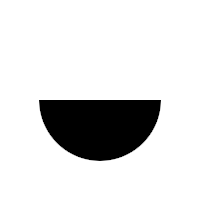
\includegraphics[width=0.32\linewidth]{../../images/binary/semicircle.png}
    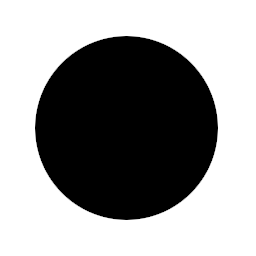
\includegraphics[width=0.32\linewidth]{../../images/binary/ellipse.png}
    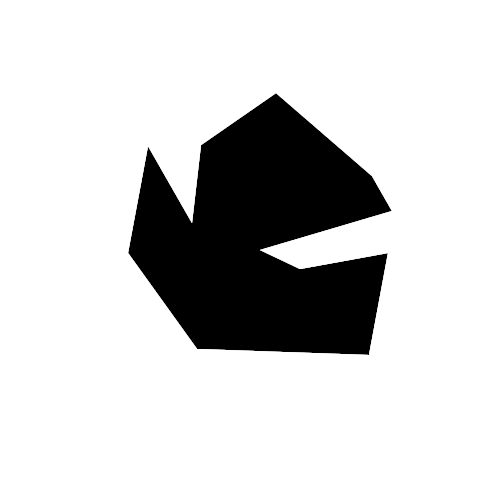
\includegraphics[width=0.32\linewidth]{../../images/binary/abstract1.png}
    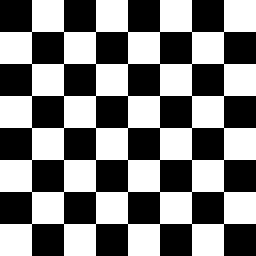
\includegraphics[width=0.32\linewidth]{../../images/binary/checkerboard32.png}
    \caption{Binary images used for testing. From left to right and from top to bottom:
        \texttt{cat}, \texttt{rect},
    \texttt{semicircle}, \texttt{ellipse}, \texttt{abstract1}, \texttt{checkerboard32},
\texttt{testlength}}\label{fig:BinaryImg}
\end{figure}

\section{Parameter Selection}\label{sec:Parameters}
As mentioned earlier, the optimal set of parameters is difficult to choose, that is why we have to
experiment a lot to find a decent approximation to this optimal set. In the following we will
therefore explain what the different parameters do, how that influences the image or mask quality
and ultimately, how we chose the parameters that we used to get our results.
First off, we talk about corner detection as this was the primary focus of our work. The parameter
choice was mainly fixed from the beginning as we used sets of parameters proven to be fairly
optimal in previous work by {<insert reference here>}. Nonetheless, we shortly go over the different
parameters and explain their influence.
\subsection{Corner Detection}
For corner detection there are not that many different parameters to play around with. In the
classical approach using the structure tensor (cf section \ref{sub:Corner}) we have only 3
parameters:
\begin{itemize}
    \item the noise scale $\sigma$
    \item the integration scale $\rho$ and
    \item a threshold parameter $T$ to filter out non-important corners
\end{itemize}
but as mentioned in section \ref{sec:Contribution}, we replaced the threshold by a percentile
parameter to make it more robust.
However, we introduced a new parameter $R$, that determines the size of the corner regions and
subsequently also the size of the region where the non-maximum suppression is performed in.

Regarding the noise scale, we generally want to choose it as large as necessary but keep it as small as
possible, meaning that we want to choose the smallest noise scale that gets rid of most of the
noise in the image since with a larger $\sigma$ 
one often faces the problem that the detected corners can not be located as accurately anymore,
since more and more relevant features are smoothed away (cf. scale space section). Another problem
is that the gaussian scale space (iterated gaussian smoothing) may even introduce new
corners.\cite{weickert96}
 Most of the time however, a $\sigma$ of 1 is sufficient enough to remove most of the noise and unnecessary
 details and still provide an accurate result.\\
Twe integration scale $\rho$ basically determines how `local' 
the corner detection is as it influences the size of the region structural information is averaged
in during the computation of the structure tensor. $\rho$ should always be chosen larger than the noise
scale $\sigma$, which leads us to a `standard' value of 2-2.5. In our experiments, these values
usually yielded the best results.\\
The newly introduced percentile parameter regulates the amount of corners that are ultimately being
detected since the percentile thresholding is applied \textit{after} the CNMS. 

\subsection{Mask radius}



\subsection{Inpainting}
The main parameters required by the inpainting process are 
\begin{itemize}
    \item the noise scale $\sigma$,
    \item the integration scale $\rho$,
    \item the contrast parameter $\lambda$, 
    \item the dissipativity parameter $\alpha$ and
    \item a non-negativity parameter $\gamma$.
\end{itemize}
The implementation of the algorithm that was provided by Joachim Weickert also requires some
technical parameters such as the choice of diffusivity function, time discretisation scheme, time
step size and iterative solver used for the semi-implicit time discretisation scheme.
 All these paramters were fixed beforehand. We used the Charbonnier diffusivity function mentioned
 in <theory>. As the other parameters are concerned, a semi-implicit scheme with a time step size
 of 1000 has been used. As an iterative solver for the system of equations that arises from the
 semi-implicit scheme a conjugate gradient solver with 200 iterations was used.
\\
If we recall from the theory section, when using EED, we do not need the integation scale, as the
integration scale only influences the radius of the structure tensor which is actually not needed
for this method of inpainting. Thus, this parameter will be fixed to 0.\\
The parameters $\alpha$ and $\gamma$ are purely numerical parameters that are used to 
stabilise the algorithm or rather help to ensure that the stencil weights of the discretisation of
the diffusion process meet certain requirements.
The choice of these parameters was set to $\alpha=0.49,\, \gamma=1.0$. In general, one could image the parameter $\alpha$ as a sharpness parameter: the larger the
$\alpha$ (but not larger than 0.5), the sharper the image. More on the nature of these two parameters can be read about in
\cite{www13, weickert96}.\\
Next up is the contrast parameter $\gamma$ that is required in the diffusivity function
\eqref{def:Diffusivity}. As already explained in the \ref{sec:Structure}, this parameter helps to
distinguish between edges and non-edges. For the EED inpainting this is especially important since
it basically determines how strongly edges will be continued into inpainting regions. We
experimented with different choices for this parameter but came to the conclusion that a fairly
small value yields the best results. In general, we used a value of 0.03 for most of the images,
but found that for a certain set of images, an even smaller value of 0.01 yielded better results.\\
Last but not least, the noise scale $\sigma$ determines how much the initial image is smoothed
before the computation of the image derivatives. In general, this parameter is always fixed at 1.0
as it only serves to regularise the differentiation process.
\section{Results}\label{sec:Results}

\begin{figure}
    \centering
    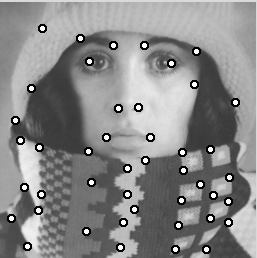
\includegraphics[width=0.31\linewidth]{../Images/trui_corners_cnms.png}
    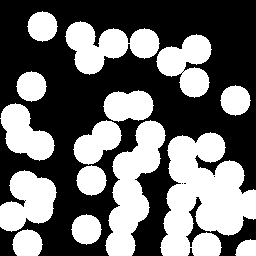
\includegraphics[width=0.31\linewidth]{../Images/trui-mask_cnms.png}
    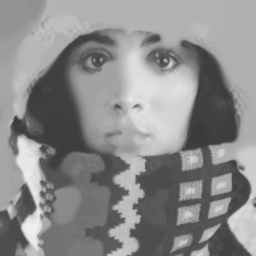
\includegraphics[width=0.31\linewidth]{../Images/trui-inpaint_cnms.png}\\
    \vspace{0.2cm}
    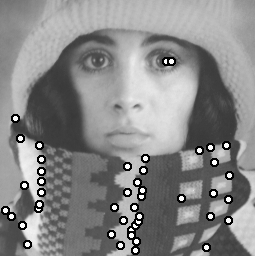
\includegraphics[width=0.31\linewidth]{../Images/trui_corners_non_cnms.png}
    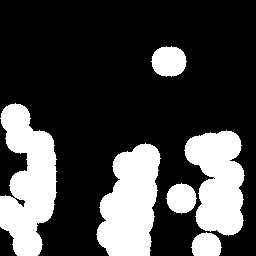
\includegraphics[width=0.31\linewidth]{../Images/trui-mask_non_cnms.png}
    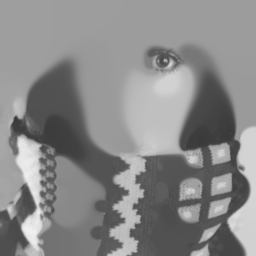
\includegraphics[width=0.31\linewidth]{../Images/trui-inpaint_non_cnms.png}
    \caption{Effect of circular non maximum suppression on spread of corners across the image.
        \textbf{Top row:} Position of corners, inpainting mask and inpainting results
        \textbf{with} CNMS.
\textbf{Bottom row:} Position of corners, inpainting mask and inpainting results \textbf{without} CNMS.
    Corner detection with Foerstner-Harris corner detector, $\sigma=1,\rho=2.5,R=15$ and a
percentile of 0.5}
\end{figure}
